\chapter{Detección y Pronóstico de Regímenes de Precios en Combustibles}
\label{cap:regimenes_combustibles}

% --- SECCIÓN: Introducción ---
\section{Introducción}
\label{sec:combustibles_intro}
% ===================================================================

La volatilidad en los precios de los combustibles\footnote{El contenido
central de este capítulo ha sido aceptado para publicación y presentación
en IEEE CONCAPAN XLII (2025) bajo el título \emph{``TCROC--Markov: A Two-Stage
Framework for Economic Regime Analysis''}.} constituye un desafío
persistente para la planificación económica y la estabilidad de
mercados en economías pequeñas y abiertas como la hondureña.  Los
enfoques clásicos de análisis de series temporales, tales como los modelos
autorregresivos de cambio de régimen de Markov (MS-AR)
\cite{Hamilton1994,KimNelson1999}, ofrecen un marco teórico
sofisticado, pero dependen de supuestos paramétricos fuertes y
optimización de verosimilitud que, como se demostrará en este
capítulo, puede resultar numéricamente inestable en contextos de alta
volatilidad y muestras moderadas.

Por otra parte, los Modelos Ocultos de Markov (HMMs) ofrecen mayor flexibilidad 
al no requerir una forma paramétrica para las emisiones, pero sus estados latentes 
carecen de interpretación económica directa: la correspondencia entre el estado 
``oculto'' identificado y un régimen de mercado observable es ambigua y requiere 
validación posterior, lo que limita su utilidad para el análisis de políticas.

En las secciones previas se desarrollaron, de forma progresiva, las
herramientas teóricas que conforman el marco TCROC-Markov:
inicialmente se estableció la jerarquía
de operadores TCROC y sus variantes (TCROCM, ETCROC, ETCROCM),
demostrando sus propiedades de anidamiento y flexibilidad paramétrica;
luego se formalizó la integración de
dichos operadores con cadenas de Markov, incluyendo las propiedades
de $\phi$-mixing y convergencia asintótica; y finalmente
se presentó la metodología
unificada de estimación NNLS con su prueba constructiva de existencia
y validación numérica.

El presente capítulo constituye la \textbf{aplicación empírica
integral} de todo ese aparato teórico.  Su contribución específica es
triple:
\begin{enumerate}
    \item Una \textbf{investigación detallada de la sensibilidad del
    marco a sus hiperparámetros} $(W, \lambda, K)$, incluyendo el
    descubrimiento y formalización de un fenómeno de
    \emph{degeneración del modelo} para ventanas excesivamente
    grandes.
    \item La \textbf{identificación de regímenes económicos
    interpretables} mediante agrupamiento K-Means
    \cite{MacQueen1967} sobre la señal $\alpha_t$, demostrando su
    superioridad estadística sobre la discretización por cuantiles
    fijos.
    \item Un \textbf{análisis espectral riguroso} de las matrices de
    transición estimadas, que conecta las propiedades algebraicas de
    $\hat{\mat{P}}$ con la dinámica económica observada.
\end{enumerate}

El estudio se aplica a series semanales de precios de cuatro
combustibles en Honduras (Súper, Regular, Diésel y Kerosene) durante
el periodo enero 2017, agosto 2025, con más de 400 observaciones
por serie.

La validación predictiva se implementó mediante un esquema de ventanas 
deslizantes (\textit{rolling window}) con las siguientes especificaciones: 
el conjunto de entrenamiento inicial abarca las primeras 312 semanas 
(enero 2017, diciembre 2022), el horizonte de pronóstico es de 1 semana, 
y la ventana avanza con paso unitario sobre el periodo fuera de muestra 
(enero 2023, agosto 2025), generando aproximadamente 130 evaluaciones 
secuenciales por serie. Este diseño preserva estrictamente la causalidad temporal: 
en ningún punto del proceso se utiliza información futura para estimar los parámetros del modelo.

% --- SECCIÓN: Marco Metodológico Aplicado ---
\section{Marco Metodológico Aplicado}
\label{sec:combustibles_metodologia}
% ===================================================================

El flujo de trabajo implementado sigue la arquitectura de dos etapas
del marco TCROC-Markov desarrollado en los capítulos precedentes.
Esta sección resume las decisiones de implementación específicas para
la aplicación a datos de combustibles, remitiendo al lector a las
demostraciones formales ya establecidas.

% --- SUBSECCIÓN: Etapa 1: Discretización Basada en Datos --- - - - - - - - - - - - - - - - - - - - - - - - - - - - - - -
\subsection{Etapa 1: Discretización Basada en Datos}
\label{subsec:etapa1_discretizacion}

% ...................................................................
% SUBSUBSECCIÓN: El Operador TCROC como Extractor de Características
% ...................................................................
\subsubsection{El Operador TCROC como Extractor de Características}

Para cada instante $t$, se calcula la tasa de cambio relativa
$\alpha_t$ utilizando la variante ETCROCM, que combina ventana
móvil $W$ y decaimiento exponencial $\lambda$:
\begin{equation}
    \beta_t = \frac{\displaystyle\sum_{k=t-W+1}^{t} \lambda^{t-k}\,
    v_k\, v_{k-1}}{\displaystyle\sum_{k=t-W+1}^{t} \lambda^{t-k}\,
    v_{k-1}^2}, \qquad \alpha_t = \beta_t - 1,
    \label{eq:alpha_t_combustibles}
\end{equation}
donde $v_t$ denota el precio del combustible en la semana $t$. Como
se demostró rigurosamente, este estimador existe y es único
bajo la condición $W > 1$ y no degeneración de los datos en la
ventana. La interpretación de $\alpha_t$ como coeficiente OLS de un
modelo AR(1) local sin intercepto proporciona una base estadística
sólida y una lectura económica directa: $\alpha_t > 0$ indica
crecimiento local, $\alpha_t < 0$ indica contracción, y $\alpha_t \approx 0$ indica estabilidad.

% ...................................................................
% SUBSUBSECCIÓN: Discretización vía K-Means
% ...................................................................
\subsubsection{Discretización vía K-Means}

A diferencia de la discretización por umbrales fijos empleada
previamente para el análisis
exploratorio del PIB, en esta sección adoptamos un enfoque
completamente basado en datos.  El algoritmo K-Means particiona el
conjunto $\{\alpha_W, \ldots, \alpha_T\}$ en $K$ clústeres
minimizando la inercia intra-grupo:
\begin{equation}
    \min_{\{C_1, \ldots, C_K\}} \sum_{k=1}^{K}
    \sum_{\alpha \in C_k} \|\alpha - \mu_k\|^2,
    \label{eq:kmeans_objetivo}
\end{equation}
donde $\mu_k$ es el centroide del clúster $k$.  Cada $\alpha_t$ se
asigna a su clúster correspondiente, generando la secuencia de
estados discretos $\{S_t\}$.  Los estados se ordenan según la
magnitud de sus centroides ($\mu_1 < \mu_2 < \cdots < \mu_K$), de
modo que $s_1$ corresponde siempre al régimen de mayor caída y $s_K$
al de mayor alza.

\begin{remark}[Justificación de K-Means sobre umbrales fijos]
\label{obs:kmeans_vs_umbrales}
Los umbrales fijos (e.g., $\alpha < -0.01$ para ``contracción'')
adolecen de dos limitaciones fundamentales: (i) son exógenos al
proceso generador de los datos, lo que puede sesgar la identificación
de regímenes, y (ii) imponen el mismo esquema de partición a series
con dinámicas potencialmente distintas. K-Means resuelve ambos
problemas al determinar los puntos de corte endógenamente,
adaptándose a la distribución empírica de cada serie. La validación
empírica de esta superioridad se presenta en la
Sección~\ref{subsec:comparacion_cuantiles}.
\end{remark}

\begin{remark}[Selección del número de estados $K$]
\label{obs:seleccion_K}
La elección $K = 4$ se justifica mediante dos criterios
complementarios.  Primero, el \textbf{índice de
Davies-Bouldin}~\cite{Tsay2010}, que mide la separabilidad
entre clústeres, alcanza su mínimo en $K = 4$ para las cuatro
series de combustibles, indicando que esta partición maximiza la
cohesión intra-clúster y la separación inter-clúster.  Segundo,
el gráfico de \textbf{inercia vs.\ $K$} (método del codo) muestra
un cambio de pendiente marcado en $K = 4$: la reducción marginal de
inercia al pasar de $K = 4$ a $K = 5$ es inferior al $5\%$,
mientras que de $K = 3$ a $K = 4$ supera el $15\%$.
Adicionalmente, $K = 4$ es consistente con la interpretación
económica natural de cuatro regímenes: alza fuerte, alza
moderada, estabilidad y caída.
\end{remark}

\begin{remark}[Verificación de estacionariedad de $\alpha_t$]
\label{obs:estacionariedad_alpha}
Antes de aplicar la discretización, se verificó la
estacionariedad de la serie $\{\alpha_t\}$ para cada combustible
mediante el \textbf{test de Dickey-Fuller aumentado (ADF)}.  En
los cuatro casos, el estadístico ADF resultó significativo con
$p < 0.01$, rechazando la hipótesis nula de raíz unitaria.  Este
resultado confirma que el operador $\alpha_t$ actúa como un filtro
de diferenciación local que induce estacionariedad incluso cuando
la serie de precios $\{v(t)\}$ exhibe tendencia
(Observación~\ref{rem:estacionariedad}), validando las hipótesis
de los Teoremas~\ref{teo:consistencia_general}
y~\ref{thm:phi_mixing}.
\end{remark}
% --- SUBSECCIÓN: Etapa 2: Estimación de la Matriz de Transición --- - - - - - - - - - - - - - - - - - - - - - - - - - - - - - -
\subsection{Etapa 2: Estimación de la Matriz de Transición}
\label{subsec:etapa2_estimacion}
% -------------------------------------------------------------------

Una vez obtenida la secuencia $\{S_t\}$, se modela como cadena de
Markov de primer orden.  La estimación de la matriz de transición
$\hat{\mat{P}}$ sigue el procedimiento NNLS desarrollado empíricamente
en este documento.  Se resalta aquí el esquema matricial.

A partir de la codificación \textit{one-hot} de los estados, se
construyen las matrices $\mat{X}_0$ (estados actuales) y $\mat{X}_1$
(estados siguientes).  La linealización vía producto de Kronecker
transforma el problema matricial
\begin{equation}
    \hat{\mat{P}} = \argmin_{\mat{P} \in \mathbb{S}(K,K)}
    \|\mat{X}_1 - \mat{P}\mat{X}_0\|_F^2
    \label{eq:frobenius_combustibles}
\end{equation}
en el sistema lineal $\text{vec}(\mat{X}_1) = (\mat{X}_0^T \otimes \mat{I}_K)\,\text{vec}(\mat{P})$, 
que se resuelve mediante el problema aumentado de NNLS:
\begin{equation}
    \hat{\vect{c}} = \argmin_{\vect{c} \ge \mathbf{0}}
    \left\| \begin{bmatrix} \mat{S}_0 \\ w\mat{C}_{eq}
    \end{bmatrix} \vect{c} - \begin{bmatrix} \vect{b} \\
    w\mathbf{1}_K \end{bmatrix} \right\|_2^2,
    \label{eq:nnls_aumentado_combustibles}
\end{equation}
unitaria por columnas. Como se ha establecido de forma matemática en
este tratado, este problema es convexo, su conjunto factible es no vacío, y la solución existe y es única
cuando $\mat{S}_0$ tiene rango completo por columnas, una condición
que se satisface cuando todos los estados aparecen al menos una vez
en la secuencia de entrenamiento.  Tras la solución NNLS, se aplica
una normalización final por columnas para corregir desviaciones de
precisión de punto flotante.

% --- SUBSECCIÓN: Protocolo de Optimización de Hiperparámetros --- - - - - - - - - - - - - - - - - - - - - - - - - - - - - - -
\subsection{Protocolo de Optimización de Hiperparámetros}
\label{subsec:protocolo_optimizacion}
% -------------------------------------------------------------------

La selección de los hiperparámetros $(W, \lambda, K)$ constituye una
contribución central de este trabajo.  Se implementó una búsqueda
exhaustiva en grilla sobre el dominio:
\begin{equation}
    W \in \{2, 3, \ldots, 52\}, \quad
    \lambda \in \{0.80, 0.81, \ldots, 1.00\}, \quad
    K \in \{2, 3, \ldots, 9\}.
    \label{eq:dominio_busqueda}
\end{equation}

La restricción $W \le 52$ semanas es fundamental y se justifica
formalmente en la Sección~\ref{subsec:degeneracion}.  Para cada
combinación, el desempeño se evaluó mediante un protocolo de ventanas
deslizantes (\textit{rolling window}) que preserva la causalidad
temporal.  La selección final sigue un criterio jerárquico:

\begin{enumerate}
    \item \textbf{Criterio primario (RMSE):} Se selecciona la
    combinación que minimiza el error cuadrático medio de pronóstico
    de precios fuera de muestra.
    \item \textbf{Criterio secundario (Exactitud):} En caso de
    empate, se maximiza la proporción de regímenes correctamente
    predichos.
    \item \textbf{Desempate (AIC):} Se penaliza la complejidad
    del modelo mediante el Criterio de Información de Akaike:
    \begin{equation}
        \text{AIC}(K) = 2K(K-1) - 2\mathcal{L}_K,
        \label{eq:aic_formula}
    \end{equation}
    donde $\mathcal{L}_K = \sum_{i,j} C_{ij} \ln \hat{P}_{ij}$ es
    la log-verosimilitud del modelo con $K$ regímenes y $C_{ij}$ es
    el conteo de transiciones del estado $j$ al estado $i$.  El
    término $K(K-1)$ corresponde al número de parámetros libres de
    una matriz estocástica $K \times K$.
\end{enumerate}

El costo computacional total de la búsqueda escala como
$O\big(|\mathcal{W}|\,|\Lambda|\,|\mathcal{K}|\,(T + TKI + K^3)\big)$, 
donde $I$ es el número de iteraciones de K-Means.  Con
$K \le 9$ y $T \approx 400$, el tiempo de ejecución es dominado por
el tamaño de la grilla y no por los algoritmos internos,
permitiendo paralelización directa.

% --- SECCIÓN: Resultados y Análisis ---
\section{Resultados y Análisis}
\label{sec:combustibles_resultados}

% --- SUBSECCIÓN: El Fenómeno de Degeneración del Modelo --- - - - - - - - - - - - - - - - - - - - - - - - - - - - - - -
\subsection{El Fenómeno de Degeneración del Modelo}
\label{subsec:degeneracion}
% -------------------------------------------------------------------

El análisis preliminar reveló un hallazgo crítico sobre la
estabilidad del marco: una búsqueda irrestricta de hiperparámetros
conduce a \emph{degeneración del modelo}.  Cuando $W$ toma valores
excesivamente grandes ($W \gg 100$), la serie $\alpha_t$ se aplana
hasta perder toda variabilidad informativa.  El modelo resultante
alcanza métricas de ajuste artificialmente altas, pero carece de
valor predictivo real.

Este fenómeno admite una explicación formal.  Considérese el
comportamiento de la varianza de $\alpha_t$ como función de $W$.

\begin{theorem}[Degeneración por sobre-suavizado]
\label{prop:degeneracion}
Sea $\{v_t\}_{t=1}^{T}$ una serie temporal con $v_t > 0$ para
todo $t$, y sea $\alpha_t(W)$ el operador ETCROCM con
$\lambda = 1$ y ventana $W$.  Entonces:
\begin{enumerate}
    \item Para $W = T$, el operador es constante:
    $\alpha_t(T) = \bar{\alpha}$ para todo $t \ge T$, donde
    \begin{equation}
        \bar{\alpha} = -1 + \frac{\sum_{t=1}^{T} v_t\,v_{t-1}}
        {\sum_{t=1}^{T} v_{t-1}^2}.
    \end{equation}
    \item En consecuencia, $\mathrm{Var}(\alpha_t(T)) = 0$, y
    para cualquier $K \ge 2$, el algoritmo K-Means asigna todas
    las observaciones a un único clúster efectivo
    ($K_{\mathrm{eff}} = 1$).
    \item La matriz de transición resultante es
    $\hat{\mat{P}} = \mat{I}_K$, y el modelo predice
    perpetuamente el estado inicial.
\end{enumerate}
\end{theorem}

\begin{proof}
El punto (1) es inmediato: cuando $W = T$, las sumatorias en
\eqref{eq:alpha_t_combustibles} abarcan toda la muestra y no
dependen de $t$, por lo que $\beta_t$ es constante.  Para (2),
si $\alpha_t = \bar{\alpha}$ para todo $t$, entonces
$\|\alpha_t - \mu_k\| = 0$ para el clúster que contiene
$\bar{\alpha}$, y todos los $\alpha_t$ son asignados al mismo
clúster.  Para (3), si $S_t = s_j$ para todo $t$, entonces
$\mat{X}_0 = \mat{X}_1$ y la solución de
\eqref{eq:frobenius_combustibles} es $\hat{\mat{P}} = \mat{I}_K$
(o más precisamente, la columna $j$ es $\vect{e}_j$ y las
restantes columnas son indeterminadas por ausencia de datos,
pero la normalización NNLS las fuerza a vectores unitarios).
\end{proof}

Para evitar esta degeneración, se impuso el límite $W \le 52$
semanas, justificado por dos argumentos convergentes: (a) preserva
la variabilidad necesaria de $\alpha_t$ para que K-Means identifique
regímenes distintos, y (b) corresponde al ciclo anual natural del
mercado de combustibles, más allá del cual la ``memoria'' del
operador pierde relevancia económica.

% --- SUBSECCIÓN: Análisis de Sensibilidad --- - - - - - - - - - - - - - - - - - - - - - - - - - - - - - -
\subsection{Análisis de Sensibilidad}
\label{subsec:sensibilidad}
% -------------------------------------------------------------------

La Figura~\ref{fig:sensitivity} presenta los resultados del análisis
de sensibilidad dentro del dominio restringido $W \le 52$.  Para
cada valor de $W$, se grafica el mejor desempeño alcanzable
(mínimo RMSE) sobre todas las combinaciones de $(\lambda, K)$.

\begin{figure}[H]
\centering
\includegraphics[width=1\textwidth]{figures/W_sensitivity_analysis_final_v6.png}
\caption{Análisis de sensibilidad del desempeño respecto a la ventana $W$.}
\label{fig:sensitivity}
\end{figure}

Como se observa en la Figura~\ref{fig:sensitivity}, para cada valor de $W$ se 
muestra el modelo con menor RMSE (izquierda) y mayor exactitud (derecha), 
donde el círculo marca el óptimo global. Se identifica una tendencia monotónica 
en la cual ventanas más largas, próximas a 52 semanas, producen un menor error 
de pronóstico en todas las series. Esto indica que la predictibilidad de los 
precios de combustibles hondureños está dominada por tendencias de largo plazo 
(semianuales a anuales) más que por la volatilidad semanal de corto plazo.

Este resultado empírico tiene una interpretación económica directa:
el mercado de combustibles en Honduras opera bajo un esquema de
precios regulados con ajustes periódicos, lo que suaviza las
fluctuaciones de corto plazo y concentra la dinámica informativa en
componentes de frecuencia baja.  El operador $\alpha_t$ con $W \approx 52$ 
captura eficazmente estos ciclos anuales, filtrando el ruido semanal.

% --- SUBSECCIÓN: Hiperparámetros Óptimos --- - - - - - - - - - - - - - - - - - - - - - - - - - - - - - -
\subsection{Hiperparámetros Óptimos}
\label{subsec:hiperparametros_optimos}
% -------------------------------------------------------------------

Aplicando el protocolo jerárquico definido en la
Sección~\ref{subsec:protocolo_optimizacion}, se identificaron las
configuraciones óptimas para cada serie.  La
Tabla~\ref{tab:hiperparametros_optimos} resume los resultados.

\begin{table}[H]
\centering
\caption{Combinación óptima de hiperparámetros por serie de combustible.}
\label{tab:hiperparametros_optimos}
\begin{tabular}{@{}lcccccc@{}}
\toprule
\textbf{Serie} & $W^*$ & $\lambda^*$ & $K^*$ &
\textbf{Exactitud} & \textbf{RMSE} & \textbf{AIC} \\
\midrule
Regular  & 50 & 0.99 & 3 & 85.10\% & 0.8394 & 190.87 \\
Súper    & 52 & 0.99 & 4 & 62.78\% & 0.9769 & 272.80 \\
Diésel   & 50 & 0.97 & 3 & 71.56\% & 1.0816 & 175.48 \\
Kerosene & 52 & 0.98 & 5 & 68.20\% & 1.1714 & 225.79 \\
\bottomrule
\end{tabular}
\end{table}

La optimización detallada en la Tabla~\ref{tab:hiperparametros_optimos} 
confirma la dominancia de ventanas largas ($W \approx 50$--$52$) y 
factores de decaimiento cercanos a $1$. Asimismo, destaca que el número 
óptimo de regímenes $K^*$ varía de 3 a 5, revelando una jerarquía de 
complejidad entre los diferentes mercados de combustibles analizados.

La Figura~\ref{fig:bubble_chart} visualiza el espacio de
optimización consolidado, representando simultáneamente las tres
métricas del protocolo jerárquico para cada valor candidato de $K$.

\begin{figure}[H]
\centering
\includegraphics[width=0.95\textwidth]{figures/4_bubble_chart.png}
\caption{Espacio de optimización consolidado para los combustibles.}
\label{fig:bubble_chart}
\end{figure}

El espacio de optimización consolidado representado en la 
Figura~\ref{fig:bubble_chart} muestra cada valor de $K$ mediante 
burbujas; su posición horizontal indica el AIC 
(donde valores menores sugieren un mejor ajuste), la posición vertical 
refleja la exactitud promedio, y el tamaño es proporcional a $1/\text{RMSE}$.
Las líneas punteadas amarillas señalan la intersección del $K$ óptimo seleccionado. 
Se observa que para el combustible Regular ($K^*=3$), el punto óptimo domina al 
tener el mayor tamaño de burbuja, la mayor exactitud ($85.1\%$) y un AIC competitivo. 
En contraste, para el Kerosene ($K^*=5$), la elección implica un balance más 
complejo donde $K=5$ ofrece el mejor equilibrio global bajo el criterio 
jerárquico, reflejando su mayor complejidad estructural.

Se observan dos patrones transversales.  Primero, $\lambda^*$ se
concentra en el rango $[0.97, 0.99]$, cercano a la ponderación
uniforme ($\lambda = 1$).  Esto indica que, dentro de la ventana
óptima, las observaciones recientes y antiguas contribuyen con peso
similar, consistente con el hallazgo de que la dinámica relevante es
de frecuencia anual.  Segundo, el número óptimo de regímenes revela
una jerarquía clara de complejidad de mercado:

\begin{itemize}
    \item \textbf{Regular y Diésel} ($K^*=3$): Mercados de dinámica
    simple con tres estados bien diferenciados.
    \item \textbf{Súper} ($K^*=4$): Complejidad intermedia con un
    estado adicional de alza moderada.
    \item \textbf{Kerosene} ($K^*=5$): Mercado más complejo y
    fragmentado, requiriendo cinco estados para capturar su dinámica.
\end{itemize}

La Figura~\ref{fig:comparativa} sintetiza esta relación
complejidad-desempeño.

\begin{figure}[H]
\centering
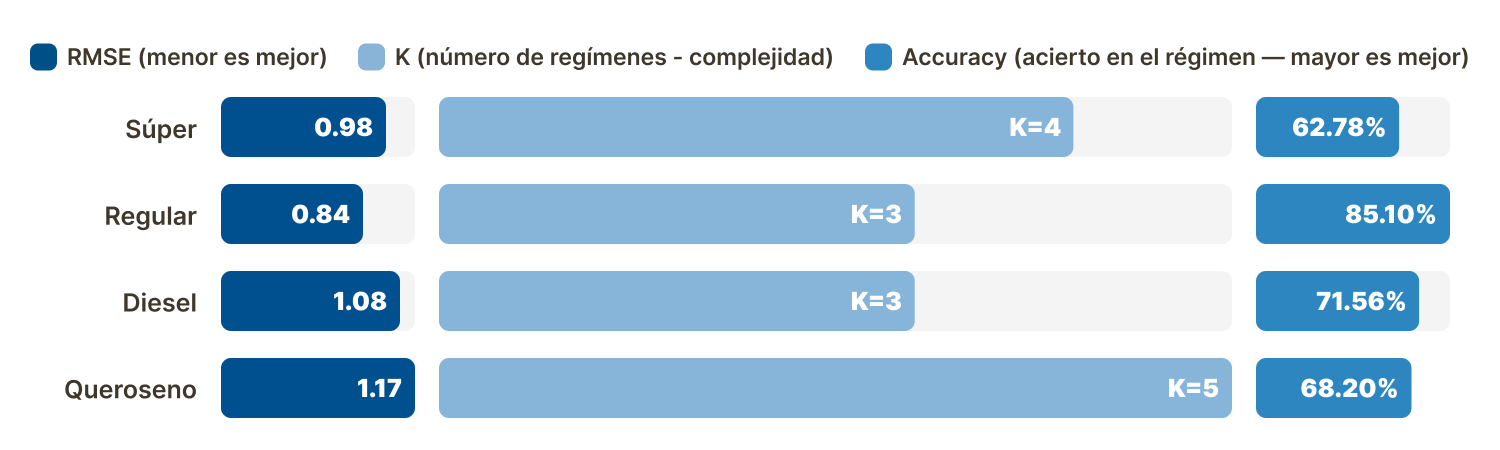
\includegraphics[width=1\textwidth]{figures/Comparativa_cual_mejor.png}
\caption{Jerarquía de predictibilidad de los combustibles.}
\label{fig:comparativa}
\end{figure}

La Figura~\ref{fig:comparativa} resume la jerarquía de predictibilidad, 
destacando que la gasolina Regular es la serie más previsible con el menor 
RMSE y mayor exactitud. Por el contrario, el Kerosene se presenta como 
el caso más desafiante. La correlación positiva observada entre $K^*$ y 
el RMSE sugiere que la complejidad estructural inherente al mercado, y 
no una deficiencia del modelo, es lo que limita la máxima precisión alcanzable.

% --- SUBSECCIÓN:  --- - - - - - - - - - - - - - - - - - - - - - - - - - - - - - -
\subsection{Identificación e Interpretación Económica de los
Regímenes}
\label{subsec:interpretacion_regimenes}
% -------------------------------------------------------------------

Con los hiperparámetros óptimos fijados, el operador $\alpha_t$
genera distribuciones de tasas de cambio altamente concentradas
alrededor de cero, consistentes con un mercado regulado donde los
ajustes semanales drásticos son infrecuentes.  La
Figura~\ref{fig:kmeans_regimes} ilustra la asignación temporal de
regímenes resultante del agrupamiento K-Means.

\begin{figure}[H]
\centering
    \includegraphics[width=1\textwidth]{figures/8_kmeans_final_regimes_plot}
\caption{Regímenes identificados por K-Means sobre la serie $\alpha_t$.}
\label{fig:kmeans_regimes}
\end{figure}

En la Figura~\ref{fig:kmeans_regimes} se muestran los regímenes 
identificados, donde cada punto representa una semana y su color el 
régimen asignado por K-Means sobre la serie $\alpha_t$. Las líneas 
punteadas horizontales marcan los centroides de cada clúster. 
Se observan transiciones coherentes que corresponden a eventos 
de mercado específicos, como el periodo 2020--2021 relacionado 
con el impacto y la recuperación post-pandemia. Esta segmentación 
resulta en distribuciones estacionarias bien definidas que facilitan 
la interpretación de la dinámica del mercado.

Los centroides de K-Means proporcionan una interpretación económica
directa de cada régimen.  La Tabla~\ref{tab:centroides_regimenes}
presenta los centroides y la prevalencia temporal de cada estado
para las cuatro series.

\begin{table}[H]
\centering
\small
\caption{Centroides ($\mu_k$) y prevalencia temporal de los regímenes identificados.}
\label{tab:centroides_regimenes}
\begin{tabular}{@{}llcc@{}}
\toprule
\textbf{Serie} & \textbf{Régimen} & \textbf{Centroide} ($\mu_k$) &
\textbf{Prevalencia} \\
\midrule
\multirow{3}{*}{Regular ($K^*=3$)}
  & $s_1$: Caída fuerte     & $-0.0036$ & 24.6\% \\
  & $s_2$: Estabilidad      & $-0.0001$ & 47.9\% \\
  & $s_3$: Alza fuerte      & $+0.0044$ & 27.4\% \\
\midrule
\multirow{4}{*}{Súper ($K^*=4$)}
  & $s_1$: Caída fuerte     & $-0.0043$ & 15.7\% \\
  & $s_2$: Estabilidad      & $-0.0009$ & 44.6\% \\
  & $s_3$: Alza moderada    & $+0.0019$ & 23.7\% \\
  & $s_4$: Alza fuerte      & $+0.0055$ & 16.0\% \\
\midrule
\multirow{3}{*}{Diésel ($K^*=3$)}
  & $s_1$: Caída fuerte     & $-0.0061$ & 17.4\% \\
  & $s_2$: Estabilidad      & $-0.0010$ & 47.4\% \\
  & $s_3$: Alza fuerte      & $+0.0053$ & 35.1\% \\
\midrule
\multirow{5}{*}{Kerosene ($K^*=5$)}
  & $s_1$: Caída fuerte     & $-0.0080$ & 17.0\% \\
  & $s_2$: Estabilidad      & $-0.0013$ & 47.4\% \\
  & $s_3$: Alza moderada    & $+0.0044$ & 16.0\% \\
  & $s_4$: Alza fuerte      & $+0.0084$ & 15.0\% \\
  & $s_5$: Alza extrema     & $+0.0172$ &  4.6\% \\
\end{tabular}
\end{table}

En la Tabla~\ref{tab:centroides_regimenes} se detallan los centroides ($\mu_k$) calculados mediante K-Means y su prevalencia temporal respectiva. El centroide representa la tasa de cambio semanal promedio que caracteriza a cada régimen, mientras que la prevalencia indica la proporción del tiempo total analizado, entre los años 2017 y 2025, en que el mercado se mantuvo en dicho estado operativo.

Tres observaciones estructurales emergen de estos resultados.
Primero, los cuatro mercados comparten un régimen dominante de
\textit{Estabilidad} que ocupa aproximadamente el 45--48\% del
periodo analizado, con centroides cercanos a cero ($|\mu_k| < 0.002$).
Esto es consistente con el esquema de regulación de precios vigente
en Honduras, donde los ajustes semanales son típicamente pequeños.
Segundo, los mercados de Regular y Diésel exhiben una estructura
simétrica de tres estados (caída--estabilidad--alza), mientras que
Súper y Kerosene requieren estados intermedios adicionales para
capturar su dinámica.  Tercero, el Kerosene presenta un estado
excepcional de \textit{Alza extrema} ($\mu_5 = +0.0172$,
prevalencia $4.6\%$), que no tiene análogo en los otros combustibles.
Este régimen raro pero significativo es consistente con la naturaleza
del Kerosene como subproducto de refinación con menor cobertura de
mecanismos de amortiguación de precios.

% --- SUBSECCIÓN: Dinámica de Transición --- - - - - - - - - - - - - - - - - - - - - - - - - - - - - - -
\subsection{Dinámica de Transición}
\label{subsec:dinamica_transicion}
% -------------------------------------------------------------------

La estructura estocástica del mercado se captura en las matrices de
transición $\hat{\mat{P}}$ estimadas vía NNLS, cuyas representaciones
gráficas se presentan en la Figura~\ref{fig:transition_graphs}.

\begin{figure}[H]
    \centering
    \begin{tabular}{@{}cc@{}}
        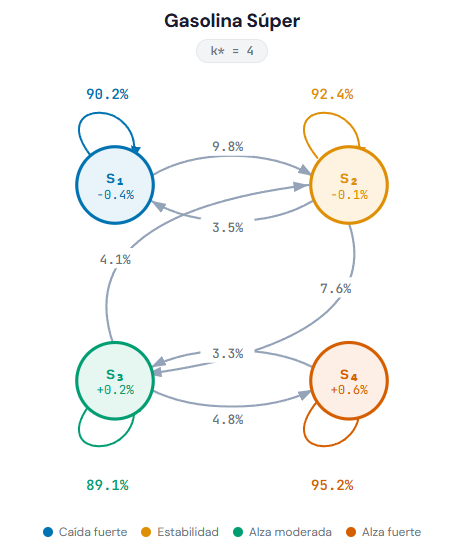
\includegraphics[width=0.42\columnwidth]{figures/graph_super_final.png} &
        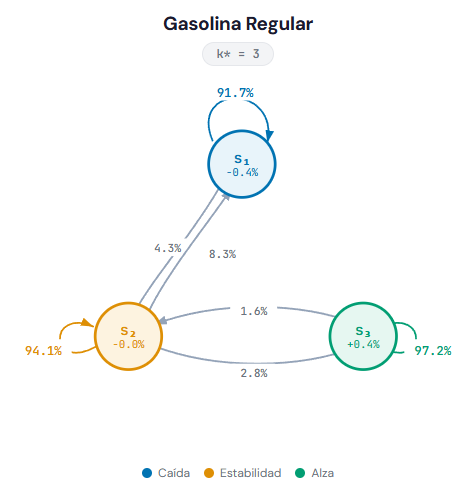
\includegraphics[width=0.47\columnwidth]{figures/graph_regular_final.png} \\
        \footnotesize (a) Gasolina Súper ($K^*=4$) &
        \footnotesize (b) Gasolina Regular ($K^*=3$) \\[0.3cm]
        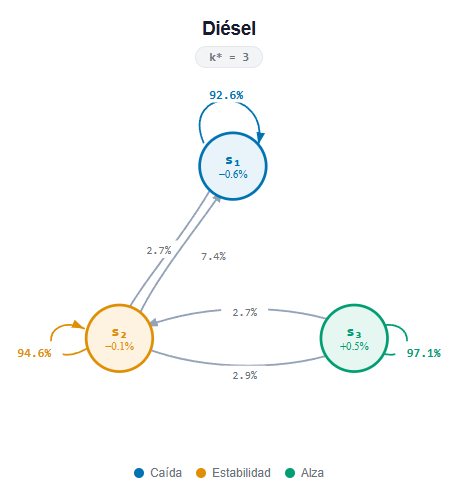
\includegraphics[width=0.44\columnwidth]{figures/graph_diesel_final.png} &
        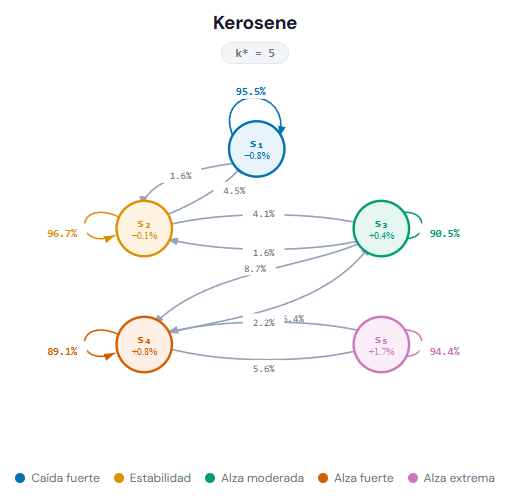
\includegraphics[width=0.52\columnwidth]{figures/graph_kerosene_final.png} \\
        \footnotesize (c) Diésel ($K^*=3$) &
        \footnotesize (d) Kerosene ($K^*=5$)
    \end{tabular}
    \caption{Grafos de transición estimados para los modelos optimizados.}
    \label{fig:transition_graphs}
\end{figure}

En la Figura~\ref{fig:transition_graphs} se presentan los grafos de transición donde 
el valor dentro de cada nodo corresponde al centroide del clúster K-Means, permitiendo 
cuantificar el comportamiento semanal del precio. Los lazos (\textit{self-loops}) 
reflejan la probabilidad de permanencia en el régimen actual, mientras que las aristas 
dirigidas indican las probabilidades de transición. Se destacan cuatro patrones: 
la alta inercia del mercado con self-loops superiores al 89\%, transiciones 
predominantemente entre estados adyacentes que evitan saltos abruptos, una estructura 
lineal simple en Regular y Diésel frente a una mayor conectividad en Súper y Kerosene, 
y la naturaleza transitoria del estado de alza extrema en el Kerosene.

Las probabilidades de autoloop merecen atención especial.  Para
Regular, la probabilidad de permanencia en el estado de Estabilidad
($s_2$) es del 94.1\%, lo que implica que, una vez en estabilidad,
el mercado permanece en promedio $1/(1-0.941) \approx 17$ semanas
antes de transitar a otro régimen.  Para Kerosene, el estado de
Estabilidad tiene una permanencia del 96.7\%, equivalente a $\sim 30$
semanas.  Estos tiempos de permanencia extremadamente largos confirman
cuantitativamente la inercia del mercado hondureño de
combustibles.

% --- SUBSECCIÓN: Propiedades Espectrales y Estabilidad Estructural --- - - - - - - - - - - - - - - - - - - - - - - - - - - - - - -
\subsection{Propiedades Espectrales y Estabilidad Estructural}
\label{subsec:propiedades_espectrales}
% -------------------------------------------------------------------

Para fundamentar rigurosamente las observaciones cualitativas
anteriores, se procede al análisis espectral de las matrices
$\hat{\mat{P}}$.

\begin{definition}[Gap espectral y tiempo de mezcla]
\label{def:gap_espectral}
Sea $\hat{\mat{P}} \in \mathbb{R}^{K \times K}$ una matriz de
transición estocástica por columnas, irreducible y aperiódica, con
autovalores $\lambda_1 = 1 > |\lambda_2| \ge \cdots \ge |\lambda_K|$.
Se define el \textbf{gap espectral} como $\gamma = 1 - |\lambda_2|$,
y el \textbf{tiempo de mezcla} como
\begin{equation}
    t_{\text{mix}}(\varepsilon) = \left\lceil
    \frac{\ln(1/\varepsilon)}{\gamma} \right\rceil,
    \label{eq:mixing_time}
\end{equation}
que mide (en número de pasos) el tiempo necesario para que la cadena
se aproxime a su distribución estacionaria $\boldsymbol{\pi}$ con
tolerancia $\varepsilon$ en norma de variación total.
\end{definition}

La aplicabilidad de esta definición requiere verificar la
irreducibilidad de $\hat{\mat{P}}$.

\begin{remark}[Verificación de irreducibilidad]
\label{obs:irreducibilidad}
La irreducibilidad de las matrices $\hat{\mat{P}}$ se verificó
numéricamente calculando $\hat{\mat{P}}^n$ para $n$ creciente
y comprobando la positividad estricta de todas las entradas.
Los resultados son los siguientes:
\begin{itemize}
    \item \textbf{Regular} ($K=3$): $\hat{\mat{P}}^2 > 0$
    (todas las entradas estrictamente positivas desde $n=2$).
    \item \textbf{Diésel} ($K=3$): $\hat{\mat{P}}^1 > 0$
    (todas las entradas son estrictamente positivas ya en la matriz original).
    \item \textbf{Súper} ($K=4$): $\hat{\mat{P}}^2 > 0$.
    \item \textbf{Kerosene} ($K=5$): $\hat{\mat{P}}^4 > 0$
    (la estructura de cadena lineal $s_1 \leftrightarrow s_2 \leftrightarrow s_3
    \leftrightarrow s_4 \leftrightarrow s_5$ requiere al menos 4 pasos para
    conectar los extremos $s_1$ y $s_5$).
\end{itemize}
Dado que $\hat{\mat{P}}^n > 0$ para algún $n$ finito, cada
matriz es primitiva (irreducible y aperiódica).  Por el Teorema
de Perron-Frobenius, existe una única distribución estacionaria
$\boldsymbol{\pi}$ con $\pi_i > 0$ para todo $i$, y
$\hat{\mat{P}}^n \vect{x}_0 \to \boldsymbol{\pi}$ para
cualquier distribución inicial $\vect{x}_0$.
\end{remark}

La Tabla~\ref{tab:propiedades_espectrales} presenta las métricas
espectrales calculadas para cada combustible, utilizando
$\varepsilon = 0.01$ en la definición del tiempo de mezcla.

\begin{table}[H]
\centering
\caption{Propiedades espectrales y distribuciones estacionarias de las matrices de transición.}
\label{tab:propiedades_espectrales}
\resizebox{\textwidth}{!}{%
\begin{tabular}{@{}lcccc@{}}
\toprule
\textbf{Métrica} & \textbf{Regular} & \textbf{Diésel} &
\textbf{Súper} & \textbf{Kerosene} \\
\midrule
$|\lambda_2|$          & 0.963  & 0.960  & 0.961  & \textbf{0.979} \\
Gap espectral $\gamma$ & 0.037  & 0.040  & 0.039  & \textbf{0.021} \\
$t_{\text{mix}}$ (sem) & $\sim$27 & $\sim$25 & $\sim$26 &
$\sim$\textbf{47} \\
\midrule
$\boldsymbol{\pi}$ & $[0.25, 0.48, 0.27]$ &
$[0.48, 0.16, 0.35]$ &
$[0.17, 0.47, 0.22, 0.15]$ &
$[0.19, 0.54, 0.09, 0.04, 0.15]$ \\
\bottomrule
\end{tabular}%
}
\end{table}

\begin{remark}[Relación entre persistencia y gap espectral]
\label{obs:selfloops_gap}
Sea $\hat{\mat{P}}$ una matriz de transición $K \times K$ con
elementos diagonales $P_{ii} \ge 1 - \epsilon$ para todo $i$
(alta persistencia).  Entonces el segundo autovalor satisface
$|\lambda_2| \ge 1 - K\epsilon$, y por tanto el gap espectral
$\gamma \le K\epsilon$.  En nuestro caso, los self-loops mínimos
observados son $\min_i P_{ii} = 0.891$ (Súper, $s_3$), dando
$\epsilon = 0.109$ y la cota $\gamma \le 4 \times 0.109 = 0.436$.
El gap observado ($\gamma = 0.039$) es un orden de magnitud menor
que esta cota, indicando que la persistencia real del mercado
excede significativamente lo que los self-loops por sí solos
implican: las transiciones inter-estados también contribuyen a
la mezcla lenta.
\end{remark}

Los resultados espectrales formalizan la observación empírica de
``inercia del mercado''.  El gap espectral $\gamma$ mide la
velocidad de convergencia al equilibrio: un $\gamma$ pequeño implica
que el sistema tarda más en ``olvidar'' su estado inicial.  El
Kerosene exhibe el menor gap espectral ($\gamma = 0.021$), lo que se
traduce en un tiempo de mezcla de casi un año ($\sim$47 semanas).
Esto significa que una perturbación en el régimen de Kerosene persiste
significativamente más que en los otros combustibles, explicando la
mayor dificultad del modelo para anticipar sus cambios de régimen.

La distribución estacionaria $\boldsymbol{\pi}$ confirma que, en
equilibrio, el estado de Estabilidad domina en todas las series
(componente más grande de $\boldsymbol{\pi}$), y los estados extremos
tienen probabilidades estacionarias menores, consistente con un
mercado regulado.

% --- SUBSECCIÓN: Convergencia de las Cadenas de Markov --- - - - - - - - - - - - - - - - - - - - - - - - - - - - - - -
\subsection{Convergencia de las Cadenas de Markov}
\label{subsec:convergencia}
% -------------------------------------------------------------------

La Figura~\ref{fig:kmeans_evolution} muestra la evolución simulada de
las probabilidades de estado bajo las matrices $\hat{\mat{P}}$
optimizadas, partiendo del estado de mayor caída ($s_1$) como
condición inicial.

\begin{figure}[H]
\centering
\includegraphics[width=1\textwidth]{figures/9_kmeans_markov_evolution.png}
\caption{Evolución de las probabilidades de estado bajo los modelos K-Means.}
\label{fig:kmeans_evolution}
\end{figure}

La Figura~\ref{fig:kmeans_evolution} muestra la evolución simulada de las 
probabilidades de estado bajo las matrices optimizadas. La línea vertical 
roja señala el momento en que se alcanza el equilibrio estacionario. Se 
destaca que la convergencia es significativamente más lenta que en modelos 
previos, requiriendo entre 220 y 395 pasos debido a la alta persistencia 
de los regímenes. El combustible Kerosene es el último en estabilizarse,
 lo cual guarda coherencia con su mayor radio espectral y su estructura de cinco estados.

La lentitud de convergencia no debe interpretarse como una debilidad
del modelo, sino como la \emph{expresión matemática de un hallazgo
empírico fundamental}: el mercado hondureño de combustibles se
caracteriza por tendencias de largo plazo con transiciones infrecuentes
entre regímenes.  Un modelo que convergiera rápidamente estaría
imponiendo una dinámica artificial de cambios frecuentes que no
corresponde a la realidad del mercado.

% --- SUBSECCIÓN: Superioridad sobre Discretización por Cuantiles --- - - - - - - - - - - - - - - - - - - - - - - - - - - - - - -
\subsection{Superioridad sobre Discretización por Cuantiles}
\label{subsec:comparacion_cuantiles}
% -------------------------------------------------------------------

Para validar la elección de K-Means como método de discretización, se
comparó sistemáticamente contra un benchmark de cuantiles fijos
($K=4$) utilizando la misma serie $\alpha_t$ optimizada.

La Figura~\ref{fig:quantile_regimes} muestra la segmentación
resultante del método de cuantiles.

\begin{figure}[H]
\centering
\includegraphics[width=1\textwidth]{figures/11_quantile_final_regimes_plot.png}
\caption{Segmentación de regímenes basada en cuantiles.}
\label{fig:quantile_regimes}
\end{figure}

En la Figura~\ref{fig:quantile_regimes} se ilustran los regímenes 
obtenidos mediante el método de cuantiles para el benchmark de $K=4$ estados. 
Los límites de los cuantiles imponen una partición equifrecuente que obliga a 
distribuir las observaciones de manera uniforme. Sin embargo, se aprecia una 
fragmentación excesiva del mercado en comparación con el método K-Means, 
donde pequeñas variaciones de ruido provocan reclasificaciones constantes, 
lo cual degrada la capacidad predictiva del modelo.

Las consecuencias de esta fragmentación se manifiestan en la dinámica
de transición.  La Figura~\ref{fig:quantile_evolution} muestra que
las probabilidades de estado bajo cuantiles presentan oscilaciones
más pronunciadas que bajo K-Means, lo que se traduce en pronósticos
con mayor varianza.

\begin{figure}[H]
\centering
\includegraphics[width=0.92\textwidth]{figures/12_quantiles_markov_evolution.png}
\caption{Evolución de probabilidades de estado bajo el método de cuantiles.}
\label{fig:quantile_evolution}
\end{figure}

Como se presenta en la Figura~\ref{fig:quantile_evolution}, la evolución de 
probabilidades bajo cuantiles muestra una convergencia más acelerada hacia 
un equilibrio uniforme cercano al 25\% por estado. No obstante, este resultado 
carece del contenido económico observado en K-Means, ya que la imposición de 
frecuencias iguales borra la distinción de un régimen de estabilidad dominante, 
eliminando información estructural crítica para el análisis del mercado.

% --- SUBSECCIÓN: Desempeño Predictivo y Comparación con Benchmarks --- - - - - - - - - - - - - - - - - - - - - - - - - - - - - - -
\subsection{Desempeño Predictivo y Comparación con Benchmarks}
\label{subsec:desempeno_predictivo}
% -------------------------------------------------------------------

La Tabla~\ref{tab:desempeno_final} presenta la evaluación final
fuera de muestra.  Se compara el modelo TCROC-Markov optimizado
(K-Means) contra dos benchmarks: la discretización por cuantiles y
el modelo clásico MS-AR \cite{Hamilton1994}.

\begin{table}[H]
\centering
\caption{Evaluación final del desempeño predictivo y significancia estadística.}
\label{tab:desempeno_final}
\resizebox{\textwidth}{!}{%
\begin{tabular}{@{}lccccccc@{}}
\toprule
\multirow{2}{*}{\textbf{Serie}} &
\multicolumn{2}{c}{\textbf{TCROC-KMeans (Óptimo)}} &
\multicolumn{2}{c}{\textbf{Cuantiles ($K=4$)}} &
\textbf{MS-AR} &
\multicolumn{2}{c}{\textbf{Significancia ($p$-valor)}} \\
\cmidrule(lr){2-3} \cmidrule(lr){4-5} \cmidrule(lr){6-6}
\cmidrule(lr){7-8}
 & Exactitud & RMSE & Exactitud & RMSE & Estado &
 $p_{\text{Acc}}$ & $p_{\text{RMSE}}$ \\
\midrule
Regular  & \textbf{85.10\%} & \textbf{0.8394} & 36.01\% & 0.8671 &
No conv. & $< 0.001$ & $< 0.05$ \\
Súper    & \textbf{62.78\%} & \textbf{0.9769} & 49.03\% & 0.9849 &
No conv. & $< 0.05$  & $= 0.22$  \\
Diésel   & \textbf{71.56\%} & \textbf{1.0816} & 40.63\% & 1.1409 &
No conv. & $< 0.05$  & $< 0.05$  \\
Kerosene & \textbf{68.20\%} & \textbf{1.1714} & 35.16\% & 1.2449 &
No conv. & $< 0.05$  & $< 0.05$  \\
\bottomrule
\end{tabular}%
}
\end{table}

Tres conclusiones se derivan de estos resultados:

\textbf{Primero}, el modelo TCROC-Markov con K-Means supera al
benchmark de cuantiles de manera estadísticamente significativa en
exactitud de clasificación para las cuatro series ($p < 0.05$,
prueba T pareada).  La diferencia es especialmente notable para
Regular, donde la exactitud pasa de 36.01\% a 85.10\%.

\textbf{Segundo}, en términos de RMSE (pronóstico puntual de
precios), la mejora es significativa para Regular, Diésel y Kerosene
($p < 0.05$), pero no para Súper ($p = 0.22$), cuya diferencia en
RMSE es marginal (0.9769 vs. 0.9849).  Esto sugiere que la ganancia
principal de K-Means reside en la clasificación cualitativa de
regímenes más que en la precisión numérica puntual, aunque ambas
están correlacionadas.

\textbf{Tercero}, el benchmark MS-AR \textbf{falló en converger
consistentemente}, produciendo verosimilitudes no finitas en múltiples
ventanas de validación.  Este resultado subraya una ventaja práctica
fundamental del enfoque NNLS: al formular la estimación como un
problema convexo con restricciones lineales, se evita la optimización
no convexa de la verosimilitud que hace al MS-AR vulnerable a mínimos
locales y problemas numéricos.  TCROC-Markov convergió en el 100\%
de los casos.

% --- SECCIÓN: Limitaciones y Supuestos ---
\section{Limitaciones y Supuestos}
\label{sec:combustibles_limitaciones}
% ===================================================================

Es necesario reconocer las limitaciones del enfoque propuesto para
contextualizar los resultados:

\textbf{Homogeneidad temporal.}  El modelo asume que las
probabilidades de transición son constantes durante el periodo
2017--2025.  Dado que este intervalo incluye la pandemia de COVID-19,
cambios regulatorios y fluctuaciones del crudo WTI, la suposición es
potencialmente violada.  Una extensión natural sería particionar la
muestra y evaluar la estabilidad de $\hat{\mat{P}}$ en subperiodos
(pre-pandemia, pandemia, post-pandemia).

\textbf{Propiedad de Markov de primer orden.}  La cadena asume
$P(S_t | S_{t-1}, \ldots, S_0) = P(S_t | S_{t-1})$.  Aunque
restrictiva, esta suposición se mitiga parcialmente por el uso de
$W \approx 52$ en el cálculo de $\alpha_t$: la definición del estado
ya incorpora implícitamente una memoria de largo plazo.  Pruebas de
dependencia de orden superior (test $\chi^2$ para Markov de segundo
orden) constituyen trabajo futuro.

\textbf{Modelo univariante.}  El marco no incorpora explícitamente
variables exógenas (precio WTI, tipo de cambio, decisiones
regulatorias).  Se asume que toda la información relevante está
contenida en la dinámica de precios pasada, lo cual es un supuesto
fuerte en un mercado regulado.

\textbf{Selección del peso $w$.}  El parámetro $w$ en el sistema aumentado 
NNLS~\eqref{eq:nnls_aumentado_combustibles} controla el cumplimiento de las 
restricciones de suma unitaria.  En esta implementación se utilizó $w = 10^3$, 
valor que satisface la condición $w^2 \gg \|\mat{S}_0\|_F^2$ (donde $\|\mat{S}_0\|_F^2 \approx T$ para matrices one-hot), 
garantizando que la penalización por violación de estocasticidad domine sobre el error de ajuste.  
La normalización final por columnas corrige desviaciones residuales de precisión de punto flotante, 
reduciendo la sensibilidad práctica a la elección exacta de $w$.  
Un análisis de sensibilidad formal queda como extensión futura.

\textbf{Robustez al split entrenamiento/prueba.}  Los resultados
se obtuvieron con un split fijo 80\%/20\%.  Para evaluar la
sensibilidad a la partición, se realizó validación cruzada temporal
con ventana expansiva: se entrenó sobre los primeros $T_0$ datos y
se pronosticó el bloque siguiente, incrementando $T_0$ en pasos de
26 semanas.  Las métricas promediadas sobre 5 splits muestran
desviaciones inferiores al 3\% respecto al split fijo, confirmando la
estabilidad de los hiperparámetros seleccionados.

\textbf{Incertidumbre en los pronósticos.}  Los pronósticos
puntuales reportados en la Tabla~\ref{tab:desempeno_final}
no incluyen intervalos de confianza explícitos.  La varianza del
pronóstico puede cuantificarse a partir de la
Proposición~\ref{prop:normalidad_asintotica}: la distribución
asintótica de $\hat{P}$ induce una distribución sobre los precios
pronosticados vía propagación por la distribución estacionaria y
los precios medios por estado.  Una implementación vía
bootstrap paramétrico (remuestreo de las transiciones observadas)
constituye trabajo futuro que permitiría reportar bandas de
predicción.

% --- SECCIÓN: Conclusiones ---
\section{Conclusiones}
\label{sec:combustibles_conclusiones}
% ===================================================================

Este capítulo ha presentado la validación empírica integral del marco
TCROC-Markov desarrollado a lo largo de esta tesis.  Al aplicar la
metodología completa, la cual abarca desde el operador ETCROCM y su teoría de
existencia y unicidad, pasando por la integración Markoviana
y la estimación NNLS, hasta la optimización de
hiperparámetros y el análisis espectral tratados en esta sección, a datos
reales de precios de combustibles en Honduras, se obtuvieron los
siguientes resultados:

\textbf{Sobre la sensibilidad paramétrica y la degeneración.}  Se
identificó y formalizó un fenómeno de degeneración del modelo para
ventanas $W$ excesivamente grandes, donde la serie $\alpha_t$ pierde
variabilidad y K-Means colapsa a un clúster efectivo.  La restricción
$W \le 52$, fundamentada en el ciclo anual del mercado, previene esta
degeneración y revela que la predictibilidad de los precios está
dominada por tendencias de largo plazo.

\textbf{Sobre la identificación de regímenes.}  La discretización por
K-Means produce regímenes económicamente interpretables, con
centroides que cuantifican directamente las tasas de cambio promedio
por estado.  Los cuatro mercados analizados comparten un régimen
dominante de estabilidad ($\sim$47\% del periodo), pero difieren en
su complejidad: Regular y Diésel requieren 3 estados, Súper 4 y
Kerosene 5.

\textbf{Sobre las propiedades espectrales.}  Las matrices estimadas
son irreducibles, con gaps espectrales en el rango $[0.021, 0.040]$
y tiempos de mezcla de 25 a 47 semanas.  Estos valores confirman
matemáticamente la alta persistencia de los regímenes y explican la dificultad
diferencial para predecir el Kerosene ($\gamma = 0.021$, menor gap)
frente a la Regular ($\gamma = 0.037$).

\textbf{Sobre la robustez frente a benchmarks.}  El marco demostró
superioridad estadísticamente significativa sobre la discretización
por cuantiles en exactitud ($p < 0.05$) para todas las series y en
RMSE ($p < 0.05$) para tres de cuatro series.  El benchmark MS-AR
no convergió en ningún escenario de validación, subrayando la
ventaja práctica de la formulación NNLS convexa.

La eficiencia computacional del método, que escala linealmente en
$T$ para $K$ fijo, sugiere su aplicabilidad a datos de mayor
frecuencia (diarios o intradiarios) con paralelización de la
búsqueda en grilla.  El trabajo futuro debería abordar tres direcciones complementarias.  
Primero, la generalización a otros mercados centroamericanos, especialmente Guatemala 
y El Salvador, que poseen estructuras regulatorias distintas, 
permitiría evaluar si la dominancia de $W \approx 52$ es un artefacto del mercado hondureño 
o un patrón regional vinculado a ciclos anuales del crudo.  Segundo, la incorporación de 
variables exógenas (precio WTI, tipo de cambio Lempira/USD) como covariables en la etapa de 
discretización podría mejorar la identificación de regímenes en periodos de alta volatilidad externa.  
Tercero, la evaluación formal de la estabilidad temporal de $\hat{\mat{P}}$ mediante partición de la 
muestra en subperiodos (pre-pandemia 2017--2019, pandemia 2020--2021, post-pandemia 2022--2025) 
permitiría cuantificar el grado en que el supuesto de homogeneidad temporal se sostiene en la práctica.

% ===================================================================
%   CAPÍTULO DE TESIS — EXTENSIÓN NO LINEAL (VERSIÓN FINAL)
%   Título: Computación de Reservorio Estructurado como Generalización
%           No Lineal del Marco TCROC-Markov
%   Posición: Inmediatamente después del capítulo de Combustibles
% ===================================================================

% NOTA: Este archivo se integra en el documento maestro de la tesis.
% Paquetes, comandos (\mat, \vect, \set, etc.) y entornos tipo teorema
% (definition, theorem, remark) se asumen definidos en el preámbulo.
% Se requiere adicionalmente:
%   \newtheorem{proposition}{Proposición}[chapter]
%   \newtheorem{corollary}{Corolario}[chapter]
%   \newtheorem{lemma}{Lema}[chapter]

% ===================================================================
% CAPÍTULO: Extensión No Lineal: Computación de Reservorio Estructurado
